\chapter{熔化与沸腾：状态变化}\label{ch:g4:changes-of-state}

你早就知道，热量能使冰融化、使水沸腾。但是
现在你有了一支\omterm{def:g3:temperature-thermometers:temperature}{温度计}——而它在融化的冰桶里
报告了一件令人惊讶的事：冰在融化的时候，
\omterm{def:g3:temperature-thermometers:temperature}{温度}\emph{纹丝不动}。让我们用新的眼光，
重新看看这些熟悉的状态变化。

\section{专有名称}

水的状态变化现在有了正式名称，适用于
每一种物质，而不只是水。由固态变为液态：
\emph{熔化}\index{熔化}。由液态变回固态：
\emph{凝固}\index{凝固}（也称固化）。由
液态变为气态：快速进行、冒大气泡时为\emph{沸腾}\index{沸腾}，
在液面上安静进行时则为\omterm{def:g2:ice-water-steam:evapcond}{蒸发}。由
气态变回液态称为液化。世界上每一种物质——
水、巧克力、铁、金——都能玩这个游戏，
只是各有各的\omterm{def:g3:temperature-thermometers:temperature}{温度}。

\begin{definition}[熔点]\label{def:g4:changes-of-state:melting-point}
物质的\emph{熔点}\index{熔点}是指
物质\omterm{def:g2:ice-water-steam:meltfreeze}{熔化}时的\omterm{def:g3:temperature-thermometers:temperature}{温度}，同时也是
\omterm{def:g3:solids-liquids-gases:liquid}{液体}\omterm{def:g2:ice-water-steam:meltfreeze}{凝固}时的\omterm{def:g3:temperature-thermometers:temperature}{温度}。水的熔点为\qty{0}{\celsius}。每
种物质都有自己的熔点：巧克力约在\qty{34}{\celsius}\omterm{def:g2:ice-water-steam:meltfreeze}{熔化}（这
与口腔\omterm{def:g3:temperature-thermometers:temperature}{温度}相近，并非偶然，问问任何一位巧克力制造商便知），石蜡约在\qty{60}{\celsius}\omterm{def:g2:ice-water-steam:meltfreeze}{熔化}，
铁则要到\qty{1538}{\celsius}才\omterm{def:g2:ice-water-steam:meltfreeze}{熔化}。
\end{definition}

\begin{definition}[沸点]\label{def:g4:changes-of-state:boiling-point}
物质的\emph{沸点}\index{沸点}是指
物质沸腾时的\omterm{def:g3:temperature-thermometers:temperature}{温度}。水的沸点为\qty{100}{\celsius}。
每种物质同样各有自己的沸点，因此细心的厨师可以
把水烧干，而同一锅中的油仍安静地保持液态。
\end{definition}

\begin{example}[用两个数读懂世界]\label{ex:g4:changes-of-state:reading}
为什么巧克力放在架子上（\qty{20}{\celsius}）是固态，
而在夏日远足时放在口袋里（\qty{35}{\celsius}）却变成了液态？原因在于，
它的\omterm{def:g4:changes-of-state:melting-point}{熔点}约为\qty{34}{\celsius}，恰好\emph{介于}这两个\omterm{def:g3:temperature-thermometers:temperature}{温度}
之间。物质在\omterm{def:g4:changes-of-state:melting-point}{熔点}以下为固态，在\omterm{def:g4:changes-of-state:melting-point}{熔点}以上为液态——
直到\omterm{def:g4:changes-of-state:boiling-point}{沸点}时变为气态。两个数字就能说清
任何物质在任何\omterm{def:g3:temperature-thermometers:temperature}{温度}下的全部情况。
\end{example}

\section{固执的温度计}

\begin{method}[正确观察冰的熔化]\label{met:g4:changes-of-state:watch}
\begin{enumerate}
  \item 在碗中放入碎冰或雪，并把
        \omterm{def:g3:temperature-thermometers:temperature}{温度计}插入其中；等待，然后读数：\qty{0}{\celsius}；
  \item 把碗移到温暖的厨房，
        每隔几分钟读取一次\omterm{def:g3:temperature-thermometers:temperature}{温度计}示数，直到冰\omterm{def:g2:ice-water-steam:meltfreeze}{熔化}；
  \item 继续读数，一直到最后一小块冰
        消失之后很久。
\end{enumerate}
结论：整个\omterm{def:g2:ice-water-steam:meltfreeze}{熔化}过程中——碗里水与冰共存时——
\omterm{def:g3:temperature-thermometers:temperature}{温度计}都固执地停在\qty{0}{\celsius}。
只有当\emph{最后一块}冰\omterm{def:g2:ice-water-steam:meltfreeze}{熔化}后，
\omterm{def:g3:temperature-thermometers:temperature}{温度}才开始上升。
\end{method}

\begin{proposition}[平台定律]\label{prop:g4:changes-of-state:plateau}
当物质发生状态变化（\omterm{def:g2:ice-water-steam:meltfreeze}{熔化}或沸腾）时，其
\omterm{def:g3:temperature-thermometers:temperature}{温度}保持不变，停在那个刻度上，无论炉子
加热得多猛烈。所输入的热量全部用于状态变化本身，
而不用于升温。固液两相共存于
\omterm{def:g4:changes-of-state:melting-point}{熔点}；液气两相共存于\omterm{def:g4:changes-of-state:boiling-point}{沸点}。
\end{proposition}

\begin{omfigure}
\begin{tikzpicture}
\begin{axis}[omaxis, width=10.5cm, height=5.6cm,
    xlabel={加热时间}, ylabel={温度 (\unit{\celsius})},
    xtick=\empty, ytick={0,100},
    ymin=-40, ymax=140, xmin=0, xmax=10]
  \addplot[very thick, omDef] coordinates
    {(0,-30) (1.5,0) (3.5,0) (5.5,100) (8.5,100)};
  \addplot[very thick, omThm] coordinates {(8.5,100) (9.6,132)};
  \node[below, font=\small] at (axis cs:2.5,-4) {冰熔化：平台};
  \node[above, font=\small] at (axis cs:7.0,103) {水沸腾：平台};
\end{axis}
\end{tikzpicture}

{\small 平稳炉火上的一锅冰，由\omterm{def:g3:temperature-thermometers:temperature}{温度计}记录：\omterm{def:g3:temperature-thermometers:temperature}{温度}
上升，冰\omterm{def:g2:ice-water-steam:meltfreeze}{熔化}时停在\qty{0}{\celsius}，
再次上升，水沸腾时停在\qty{100}{\celsius}，
直至烧干。（最后的红色上升段表示水蒸气。）}
\end{omfigure}

\begin{omfigure}
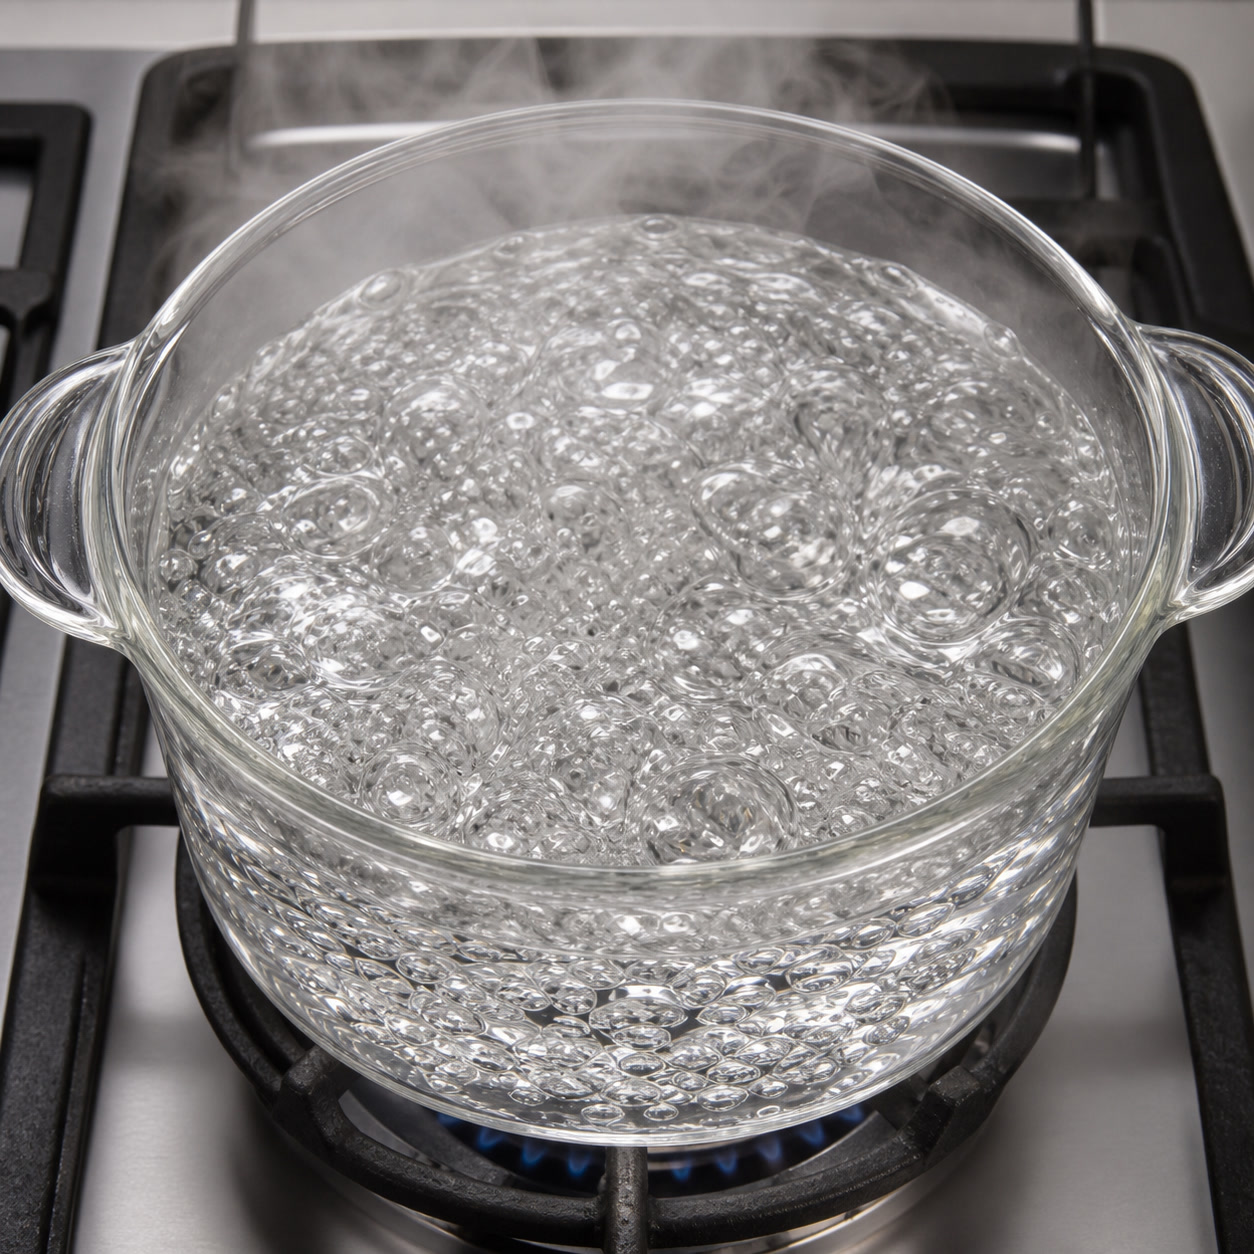
\includegraphics[width=0.45\linewidth]{images/book1/ai/g4-changes-boiling-pot.jpg}

{\small 剧烈沸腾：气泡在\omterm{def:g3:solids-liquids-gases:liquid}{液体}内部形成，并在表面破裂——而\omterm{def:g3:temperature-thermometers:temperature}{温度计}始终停在\omterm{def:g4:changes-of-state:boiling-point}{沸点}。}
\end{omfigure}

\begin{example}[厨房里的平台]\label{ex:g4:changes-of-state:kitchen}
这就是为什么微沸与剧烈沸腾的水煮面条速度一样快：
两锅水都恰好处于\qty{100}{\celsius}——猛火的那一锅
只是把多余的热量用于更快地产生水蒸气。另外，
这也解释了为什么加了冰块的饮料会一直保持\qty{0}{\celsius}，
直到最后一小块冰融化：正在融化的冰把\omterm{def:g3:temperature-thermometers:temperature}{温度}
牢牢固定在那个刻度上。
\end{example}

\begin{remark}[眼睛看不见的数字]\label{rem:g4:changes-of-state:invisible}
没有\omterm{def:g3:temperature-thermometers:temperature}{温度计}，谁也猜不到这个平台：锅里看起来
越来越热闹，冰桶看起来越来越平静，而两者的
\omterm{def:g3:temperature-thermometers:temperature}{温度}都纹丝不动。这又是一次\omterm{def:g2:measuring-length:measure}{测量}战胜表象的
胜利，也是仪器交给科学的最早
重大惊奇之一。
\end{remark}

\section{每种物质都保有自己的标志温度}

\begin{proposition}[标志温度是物质的身份标识]\label{prop:g4:changes-of-state:identity}
纯净物质的\omterm{def:g4:changes-of-state:melting-point}{熔点}和\omterm{def:g4:changes-of-state:boiling-point}{沸点}永远不变：
水在\qty{0}{\celsius}\omterm{def:g2:ice-water-steam:meltfreeze}{熔化}，无论是今天还是明天，无论是在宫殿里
还是在帐篷中。标志\omterm{def:g3:temperature-thermometers:temperature}{温度}是物质身份的一部分，保持得
如此稳定，以至于科学家只要\omterm{def:g2:measuring-length:measure}{测量}未知物质在何\omterm{def:g3:temperature-thermometers:temperature}{温度}\omterm{def:g2:ice-water-steam:meltfreeze}{熔化}、沸腾，
就能识别这种物质。
\end{proposition}

\begin{example}[蜡烛与铸造厂]\label{ex:g4:changes-of-state:foundry}
壁炉旁的蜡烛软塌下来、不断滴落：蜡在
约 \qty{60}{\celsius} 时越过\omterm{def:g4:changes-of-state:melting-point}{熔点}。在铸造厂里，工人把发出橙红色光的
液态铁水像汤一样倒出来——他们的熔炉已超过
\qty{1538}{\celsius}。同样的游戏，标志\omterm{def:g3:temperature-thermometers:temperature}{温度}却天差地别：壁炉能对蜡做的事，
只有熔炉才能对铁做到。而金在 \qty{1064}{\celsius} \omterm{def:g2:ice-water-steam:meltfreeze}{熔化}：
金匠们几千年来一直知道这个数字，
即便不用度数表示，而是凭手上的经验。
\end{example}

\begin{omfigure}
\begin{tikzpicture}[scale=0.85]
  \draw[-Stealth, very thick] (0.5,0) -- (11.2,0);
  \node[right, font=\small] at (11.15,0.4) {越热};
  \foreach \x/\t/\name in {1.3/0/{冰融化}, 3.1/34/{巧克力},
      4.4/60/{蜡}, 6.2/100/{水沸腾}, 8.3/1064/{金},
      10.1/1538/{铁}} {
    \draw[thick] (\x,-0.12) -- (\x,0.12);
    \node[above, font=\footnotesize] at (\x,0.2) {$\t$};
    \node[below, font=\footnotesize, align=center] at (\x,-0.2) {\name};
  }
\end{tikzpicture}

{\small 几种日常物质的标志\omterm{def:g3:temperature-thermometers:temperature}{温度}，以\omterm{def:g3:temperature-thermometers:temperature}{摄氏度}计（图中
横轴已压缩——铁的标记实际上比水的远十五倍）。
每种物质始终带着自己的数字。}
\end{omfigure}

\section{练习}

\begin{exercise}[$\star$]\label{exo:g4:changes-of-state:1}
写出下列变化的名称：固态变为液态；\ 液态变为固态；\ 液态
在沸腾时变为气态；\ 气态在冷窗户上变为液态。
\end{exercise}

\begin{exercise}[$\star$]\label{exo:g4:changes-of-state:2}
水的两个标志\omterm{def:g3:temperature-thermometers:temperature}{温度}分别是多少？并且
巧克力的\omterm{def:g4:changes-of-state:melting-point}{熔点}大约是多少？
\end{exercise}

\begin{exercise}[$\star$]\label{exo:g4:changes-of-state:3}
一只碗里盛着冰和水的混合物，充分搅拌后，
\omterm{def:g3:temperature-thermometers:temperature}{温度计}的读数是多少？若仍有少量冰未化完，
五分钟后\omterm{def:g3:temperature-thermometers:temperature}{温度计}的读数会是多少？
\end{exercise}

\begin{exercise}[$\star$]\label{exo:g4:changes-of-state:4}
叙述平台规律。水在沸腾时，炉子的热量去哪里了？
既然\omterm{def:g3:temperature-thermometers:temperature}{温度}不再继续上升？
\end{exercise}

\begin{exercise}[$\star$]\label{exo:g4:changes-of-state:5}
蜡在 \qty{60}{\celsius} 附近\omterm{def:g2:ice-water-steam:meltfreeze}{熔化}。蜡烛在
\qty{20}{\celsius} 的客厅里是固态还是液态？\ 紧挨着把它烤到
\qty{80}{\celsius} 的火焰旁？\ 在 \qty{35}{\celsius} 的夏日阁楼里？
\end{exercise}

\begin{exercise}[$\star$]\label{exo:g4:changes-of-state:6}
意大利面在微沸的水中煮制。爸爸把火调到
最大，锅里的水剧烈翻滚。现在水的\omterm{def:g3:temperature-thermometers:temperature}{温度}更高了吗？
多出的热量转而产生了什么？
\end{exercise}

\begin{exercise}[$\star$]\label{exo:g4:changes-of-state:7}
在本章的平台图上，你如何
不读一个字就能找出两次状态变化？
\end{exercise}

\begin{exercise}[$\star$]\label{exo:g4:changes-of-state:8}
铁在 \qty{1538}{\celsius} \omterm{def:g2:ice-water-steam:meltfreeze}{熔化}，金在 \qty{1064}{\celsius} \omterm{def:g2:ice-water-steam:meltfreeze}{熔化}。
一座熔炉的\omterm{def:g3:temperature-thermometers:temperature}{温度}保持在 \qty{1200}{\celsius}：两种金属中哪一种
在其中会像汤一样流动，哪一种仍是\omterm{def:g3:solids-liquids-gases:solid}{固体}？
熔炉\omterm{def:g3:temperature-thermometers:temperature}{温度}比另一种金属的\omterm{def:g4:changes-of-state:melting-point}{熔点}相差多少度？
\end{exercise}

\begin{exercise}[$\star$]\label{exo:g4:changes-of-state:9}
为什么加了冰块的饮料直到最后一小片冰都一样凉，
只有等冰全部融化后，才开始升温？
\end{exercise}

\begin{exercise}[$\star\star$]\label{exo:g4:changes-of-state:10}
一位科学家收到一种未知的白色\omterm{def:g3:solids-liquids-gases:solid}{固体}。她发现它恰好在
\qty{0}{\celsius} \omterm{def:g2:ice-water-steam:meltfreeze}{熔化}，其\omterm{def:g3:solids-liquids-gases:liquid}{液体}恰好在
\qty{100}{\celsius} 沸腾。她最可能推断这是什么物质？
又是哪一条规律使标志\omterm{def:g3:temperature-thermometers:temperature}{温度}可以充当物质的“身份证”？
\end{exercise}

\begin{exercise}[$\star\star$]\label{exo:g4:changes-of-state:11}
登山者报告说，在高大山峰的高处，水会沸腾，
但水只是\emph{刚刚}烫得碰不得，而他们的茶
始终泡不好。日常生活中关于沸水的哪一个确定无疑的认识
在高处会失效？（原因就藏在\omterm{def:g2:air-around-us:air}{空气}本身之中，
后面关于气压的一章将揭示它。）
\end{exercise}
